\section{Simulated Results}
%Previously we defined good paths in terms of the actual cost of the path in relation to the costmap. However, these metrics are not necessarily the ones we ultimately want to use when we move up to an interaction mindset. 

%\subsubsection{Path Length}
%\subsubsection{Closest Approach Distance}
%\subsubsection{Average Distance to Obstacle}

%If we were simply to accept the path with the lowest total cost as ``the best,'' we could now rest, assured that Dijkstra's algorithm would find the optimal path. However, in robotics, and particularly human robot interaction, there are other metrics that weigh on the value of a path. The one that is of most use to us here is the closest distance between the path and the obstacle. With the bracket shape we discussed earlier, that metric has the value of $\yhat$. There are many other metrics that we could consider, including the path length and the average distance from path to obstacle, however, those measures work proportionally to the closest distance in all of the cases considered here. A further analysis of different path metrics is considered in the Future Work section. 

Given the estimates and approximations that were needed to mathematically explain some of the properties of the Gaussian non-lethal obstacles, to fully understand their behavior, we must actually run the path planning algorithms. Costmaps were set up using the general scenario described in Problem Statement section and with the functions described below. For each set of parameters, a path was planned and the closest distance / $\yhat$ was calculated. 

For the flat non-lethal obstacle, we found that the derived paths followed the exact pattern set up by our inequality. For instance, a $5\times6$ constant valued obstacle ($w=5$) required traversing six extra cells to go around ($h=6$) and when the path constant was fifty ($P=50$), the amplitude required to force the algorithm to chose a path that went through the obstacle was $A<60$, i.e. the solution to equation (6). All amplitudes less than 60 resulted in the straight path, and all greater than 60 resulted in the path that goes around. When $A=60$, the two paths have equal cost, but only one is returned.

\begin{figure}
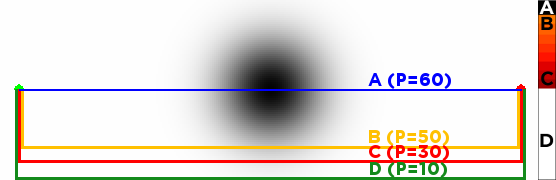
\includegraphics[width=\columnwidth]{graphix/SomePaths.png}
\caption{Paths around a Gaussian with Varying Path Constant - As $P$ decreases from (A) to (D), the path gets further and further away from the nonlethal obstacle, reflecting the length of the path becoming less important.}
\label{fig:somepaths}
\end{figure}

For the Gaussian non-lethal obstacle, the results of the simulation are a bit more complex. We know that there are certain values of parameters that result in specific behaviors, which we can see from Figure \ref{fig:colormaps}. For instance, according to equation (2), if $P/A$ is too high, there will be no solution and the optimal path will be at $\yhat=0$. We can see this in all four graphs of Figure \ref{fig:colormaps}, in that there are black areas (representing $\yhat=0$) for the large values of P and small values of A. We can also see in Figure \ref{fig:gap} that P and A have a linear relationship, which means that as long as the ratio of $P:A$ remains constant, the value of $\yhat$ will remain constant as well (given a particular variance). 

The relationship between variance and $\yhat$ is a bit more complicated, which is logical given equation (2). For any given finite positive value of $\yhat$ we can decrease the variance to get a smaller $\yhat$. This can be seen in Figure \ref{fig:gvp} for instance, where you can pick any colored point and move to a lesser variance (to the left) and get a lower $\yhat$. However, the extent to which decreasing the variance will decrease $\yhat$ depends on the other variables. 

Conversely, increasing the variance (moving to the right) can result in multiple behaviors. As expected, increasing the variance will move the closest distance as far away as possible, until it hits the border of the grid. This edge behavior can be seen in the white area on the bottom right portion of Figure \ref{fig:gvp}. At these values, the path is the maximal distance it can be away from the obstacle while still in the bounds of the grid. However, for the top portion of that figure, increasing the variance can actually \emph{decrease} the closest distance, all the way to $\yhat=0$. This corresponds with the fact that $ \sqrt{\frac{\pi}{2\sigma^2}} \yhat \exp\Big( \frac{-\yhat^2}{2\sigma^2} \Big) $ approaches 0 as $\sigma$ increases, which means that $P/A$ needs to have even smaller values to ensure a positive finite solution. 

Lastly, it is worth noting that the relationship between amplitude and path constant is a key contributor to the ease of tuning parameters. Consider Figure \ref{fig:gav} where $P=10$ and Figure \ref{fig:gav2} where $P=25$. When $P$ is relatively low, there are many valid parameter combinations to get positive $\yhat$. However, with a higher $P$, there are significantly fewer options. In some cases, it does not matter what variance you dial in, $\yhat$ will not change from being 0. 

\newcommand{\szsz}{.42}
\begin{figure}[t]
\centering
\subfloat[Amplitude vs. Path Constant]{
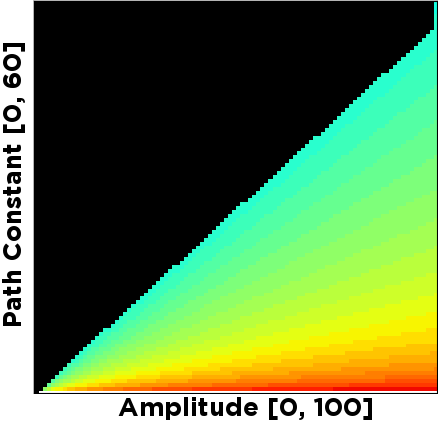
\includegraphics[width=\szsz\columnwidth]{graphix/gap.png}
\label{fig:gap}}
\qquad
\subfloat[Variance vs. Path Constant]{
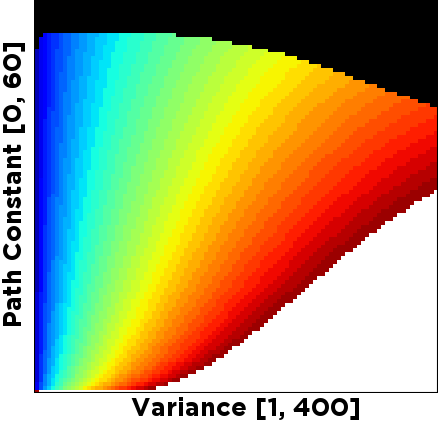
\includegraphics[width=\szsz\columnwidth]{graphix/gvp.png}
\label{fig:gvp}}\\
\subfloat[Amplitude vs. Variance \newline($P=10$)]{
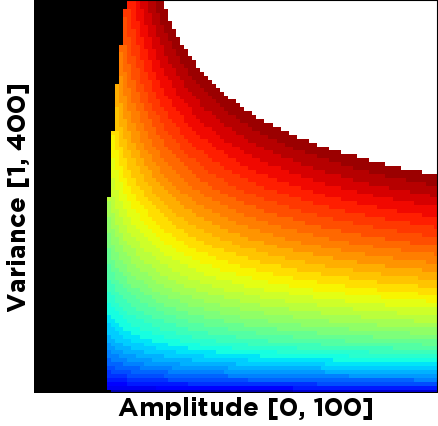
\includegraphics[width=\szsz\columnwidth]{graphix/gav.png}
\label{fig:gav}}
\qquad
\subfloat[Amplitude vs. Variance \newline($P=25$)]{
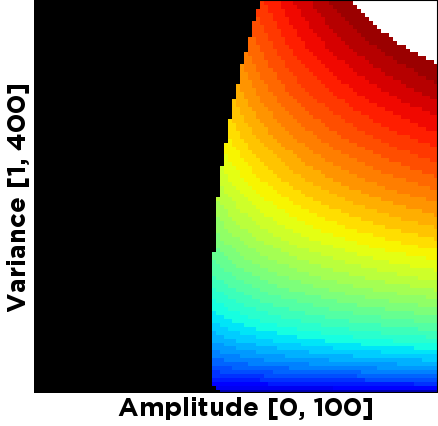
\includegraphics[width=\szsz\columnwidth]{graphix/gav2.png}
\label{fig:gav2}}
\caption{Heat Maps of $\yhat$ for different parameters for a Gaussian obstacle- The black areas mark where the path goes straight through the obstacle ($\yhat=0$), i.e. where the path constant is too high or the amplitude is too low. The white areas mark where the optimal path is as far away from the obstacle ($\yhat=\infty$), i.e. where the path traces the outer boundaries of the grid. Everything else is where $\yhat$ has a positive finite value, color coded with red paths being the longest and blue paths being the shortest.}
\label{fig:colormaps}
\end{figure}

